\documentclass[a4paper,12pt]{article}

\usepackage[section]{placeins}
\usepackage[czech]{babel}
\usepackage[utf8]{inputenc}
\usepackage[T1]{fontenc}
\usepackage{hyperref}
\usepackage{enumitem}
\usepackage{mathrsfs}
\usepackage{amsmath}
\usepackage{amssymb}
\usepackage{rotating}
\usepackage{graphicx}
\usepackage{pgfplots}
\usepackage{tikz}
\usepackage{siunitx}
\usepackage{booktabs}
\usepackage{subcaption}
\usepackage{algorithm}
\usepackage{algorithmic}
\usepackage{geometry}

\usepackage{listings}
\usepackage{xcolor}

\definecolor{codegreen}{rgb}{0,0.6,0}
\definecolor{codegray}{rgb}{0.5,0.5,0.5}
\definecolor{codepurple}{rgb}{0.58,0,0.82}
\definecolor{backcolour}{rgb}{0.95,0.95,0.92}

\lstdefinestyle{mystyle}{
    backgroundcolor=\color{backcolour},   
    commentstyle=\color{codegreen},
    keywordstyle=\color{magenta},
    numberstyle=\tiny\color{codegray},
    stringstyle=\color{codepurple},
    basicstyle=\ttfamily\footnotesize,
    breakatwhitespace=false,         
    breaklines=true,                 
    captionpos=b,                    
    keepspaces=true,                 
    numbers=left,                    
    numbersep=5pt,                  
    showspaces=false,                
    showstringspaces=false,
    showtabs=false,                  
    tabsize=2
}

\lstset{style=mystyle}

\newgeometry{vmargin={40mm}, hmargin={25mm,25mm}}
\renewcommand\refname{Literatura}

\pgfplotsset{
    compat=1.9, 
    % width=\linewidth
    /pgfplots/ybar legend/.style={
    /pgfplots/legend image code/.code={%
        \draw[##1,/tikz/.cd,yshift=-0.25em]
        (0cm,0cm) rectangle (3pt,0.8em);},
    },
    /pgf/number format/use comma,
    /pgf/number format/1000 sep={\ }
}
\pgfplotsset{%
    axis line origin/.style args={#1,#2}{
        x filter/.append code={ % Check for empty or filtered out numbers
            \ifx\pgfmathresult\empty\else\pgfmathparse{\pgfmathresult-#1}\fi
        },
        y filter/.append code={
            \ifx\pgfmathresult\empty\else\pgfmathparse{\pgfmathresult-#2}\fi
        },
        xticklabel=\pgfmathparse{\tick+#1}\pgfmathprintnumber{\pgfmathresult},
        yticklabel=\pgfmathparse{\tick+#2}\pgfmathprintnumber{\pgfmathresult}
    }
}


\author{Bc. Vojtěch Moravec}
\title{Klasifikace psů podle plemen}
\date{LS 2020}

\newcommand{\image}[4]{\begin{figure}[ht!] \centering \includegraphics[width=#4\linewidth]{Figures/#1} \caption{#2} \label{#3} \end{figure}}
\newcommand{\imageSDW}[4]{\begin{sidewaysfigure} \centering \includegraphics[width=#4\linewidth]{Figures/#1} \caption{#2} \label{#3} \end{sidewaysfigure}}

\begin{document}
\maketitle
\newpage
% \tableofcontents
% \newpage

\section{Úvod}
V tomto projektu do předmětu Metody Analýzy Dat 4 se budeme zabývat kategorizací neboli klasifikací obrazových dat. Přesněji se zaměříme na kategorizaci psů podle plemen. Toto téma jsme zvolili podle úkolu ze stránky Kaggle, který můžeme nalézt na adrese \linebreak \url{https://www.kaggle.com/c/dog-breed-identification/overview/description}.  \linebreak Cílem tohoto úkolu je pomocí trénovacích dat naučit klasifikátor, který bude následně schopen kategorizovat obrázky psů do 120 vybraných plemen. Jelikož se jedná o obrazová data a klasifikaci, tak jsme se rozhodli využít konvolučních sítí s mnoha vrstvami, které jsou v současnosti \emph{state of the art} metodou pro klasifikaci a detekci objektů v obrazových datech. V této práci nejprve uvedeme informace o originálních datech a jak jsme je zpracovali. Následně se budeme zabývat samotnou klasifikací a výsledky.

\section{Popis datasetu}
Dataset, který je k dispozici k úkolu na stránce Kaggle (viz URL v předchozí kapitole), vychází z datasetu psů vytvořeného na Standfordské univerzitě. Konkrétně se jedná \linebreak o \emph{Stanford Dogs Dataset} \cite{KhoslaYaoJayadevaprakashFeiFei_FGVC2011}. Kde tento dataset byl vytvořen z ještě většího datasetu ImageNet \cite{imagenet_cvpr09}.

Originální úkol na stránce Kaggle obsahuje jak trénovací, tak i testovací dataset, ale labely jsou k dispozici jen pro trénovací dataset. Label je pravdivá hodnota, která nám říká, do které kategorie obrázek spadá. Konkrétně jaké je plemeno psa na daném obrázku. Absence testovacích labelů, znamená nemožnost vyhodnotit naše modely. Proto jsme se rozhodli využít originální \emph{Stanford Dogs Dataset}, ve kterém nalezneme pro všechny obrázky labely. Četnosti jednotlivých psích plemen v trénovacím datasetu jsou pro všechny plemena rovny hodnotě 100. Pro jedno plemeno je tedy vždy k dispozici 100 trénovacích obrázků. Velikost celého trénovacího datasetu je 12000 obrázků. Četnosti v testovacím datasetu se již liší a najdeme je na Obrázku~\ref{fig:test_breed_dist}. Počet 100 obrázků na jedno plemeno je dosti malý, vzhledem k tomu, že chceme kategorizovat celkem 120 plemen. V této práci vyzkoušíme několik strategií, jak se s tímto vypořádat. Nejprve vybereme pouze 20 plemen, které jsou nejčastější v testovacím datasetu. Poté také vyzkoušíme umělé zvětšení datasetu pomocí augmentace dat a hlavně se zaměříme na \emph{transfer learning}.

\image{test_distribution.pdf}{Četnost jednotlivých plemen v testovacím datasetu}{fig:test_breed_dist}{0.65}

\subsection{Příprava datasetu}
V \emph{Stanford Dogs Dataset} jsou pro nás důležité soubory \texttt{images.tar} a \texttt{lists.tar}. První archív obsahuje po rozbalení obrázky psů, rozdělených do podsložek podle plemen. Trénovací i testovací data jednoho plemene jsou tedy uloženy v jedné složce. Druhý archív obsahuje binární soubory v MATLAB formátu.
Konkrétně se jedná o \texttt{train\_list.mat}, resp \texttt{test\_list.mat}, tyto soubory obsahují cesty k trénovacím, resp. testovacím obrázkům a zároveň jejich labely. Již upravené soubory budou k dispozici v přílohách této práce, jedná se o:

\begin{itemize}
    \item \texttt{classes.csv} - Seznam všech tříd a příslušících číselných labelů
    \item \texttt{train.csv} - Seznam obrázků, které jsou využity k trénování, spolu s labely
    \item \texttt{test.csv} - Seznam obrázků, které jsou využity k testování, spolu s labely
\end{itemize}

Co se týče předzpracování dat, před samotným učením, tak my jsme provedli pouze sjednocení velikosti obrázků a normalizaci. Obrázky, ať už v trénovací nebo testovací množině, měli různé rozměry. Konvoluční síť má na vstupu definován rozměr vstupních dat, proto museli být rozměry obrázků sjednoceny. Rozhodli jsme se použít rozměr\linebreak $300 \times 300 \times 3$, neboli obraz 300 pixelů vysoký a široký se třemi barevnými kanály. Obrázky jsme nepřeváděli do stupňů šedi, neboť si myslíme, že barevná složka je poměrně důležitým faktorem, při klasifikaci psího plemena.

Normalizace byla provedena z rozsahu pixelů $[0;255]$ na $[0;1]$. Celé načtení datasetu, spolu se změnou velikosti a normalizací bylo provedeno následující funkcí, za pomocí dvou funkcí \texttt{load\_img} a \texttt{img\_to\_array} z Python knihovny Keras \cite{chollet2015keras}.

\begin{lstlisting}[language=Python]
IMG_DIM = 300
def load_image_dataset(folder, paths):
    dataset = []
    count = len(paths)
    for i in range(count):
        imagePath = os.path.join(folder, paths[i])
        image = load_img(imagePath,target_size=(IMG_DIM,IMG_DIM))
        dataset.append(img_to_array(image,dtype=np.float32) / 255)
    return np.asarray(dataset)
\end{lstlisting}


Ukázku obrázků z datasetu můžeme vidět na Obrázku \ref{fig:dataset_example}. Pod každým obrázkem nalezneme název třídy, do které spadá, tedy psí plemeno.
\image{datasat_example.pdf}{Ukázka z datasetu}{fig:dataset_example}{1.0}

\newpage
\section{Klasifikace 20 plemen}
V této kapitole se zaměříme na klasifikaci 20 nejčastějších plemen v testovacím datasetu, jejich četnosti můžeme vidět na Obrázku \ref{fig:t20_test_dist}.

\image{t20_test_breeds.pdf}{Četnost 20 nejčetnějších plemen v testovacím datasetu}{fig:t20_test_dist}{1}

V trénovacím datasetu se stále nachází 100 obrázků na jedno plemeno, a proto je velikost trénovací sady 2000 obrázků. Z důvodu malé velikosti, jsme vzali pouze 10\% této sady na validační dataset. První model, který jsme vyzkoušeli a taky největší, který nám dovolili hardwarové limitace paměti, je tento:
\begin{lstlisting}[language=Python]
model = keras.Sequential(layers=[
    Input(shape=(IMG_DIM, IMG_DIM, 3), dtype=np.float32), # 300 x 300
    Conv2D(64,kernel_size=(5,5),activation='relu',),
    Conv2D(64,kernel_size=(5,5),activation='relu'),
    Dropout(rate=0.15),
    Conv2D(64,kernel_size=(5,5),activation='relu'),       
    MaxPooling2D(pool_size=(2,2)),                       # 150 x 150  
    Conv2D(64,kernel_size=(5,5),activation='relu'),
    Conv2D(64,kernel_size=(5,5),activation='relu'),
    MaxPooling2D(pool_size=(2,2)),                       # 75 x 75
    Conv2D(128,kernel_size=(5,5),activation='relu'),
    Dropout(rate=0.15),
    Conv2D(128,kernel_size=(5,5),activation='relu'),
    Conv2D(128,kernel_size=(5,5),activation='relu'),
    MaxPooling2D(pool_size=(2,2)),                       # 37 x 37  
    Conv2D(256,kernel_size=(3,3),activation='relu'),
    Conv2D(256,kernel_size=(3,3),activation='relu'),
    MaxPooling2D(pool_size=(2,2)),                       # 18 x 18
    Conv2D(256,kernel_size=(3,3),activation='relu'),
    Conv2D(256,kernel_size=(3,3),activation='relu'),
    MaxPooling2D(pool_size=(2,2)),                       # 9 x 9
    GlobalMaxPooling2D(),
    Dense(units = CLASS_COUNT, activation='softmax')
])
\end{lstlisting}

V tomto modelu můžeme vidět bloky konvolučních vrstev, následovány MaxPooling2D vrstvou. MaxPooling2D vždy snižuje rozměry výstupu vrstvy dvojnásobně.  Tyto rozměry jsou uvedeny v komentářích na pravé straně. Jako poslední je plně propojená vrstva, kde počet neuronů je roven počtu klasifikovaných tříd, v tomto případě tedy 20. Důležitá je aktivační funkce \texttt{softmax} v poslední vrstvě, která vlastně generuje pravděpodobnosti jednotlivých tříd. Co se týče ztrátové funkce, tak tento model a spolu s ním všechny modely, které budou uvedeny v této práci, používá \emph{sparse categorical crossentropy}. Tato funkce je zvolena, neboť jednotlivé třídy jsou exkluzivní a pes by měl být pouze jednoho plemene. \emph{Nechceme-li detekovat křížence, což není cílem této práce.} Stejně tak v celé práci je zvolen optimizátor \emph{Adam}, úspěšnost měříme pomocí přesnosti a v základu trénujeme ve 20 epochách.

Výsledky trénování první konvoluční neuronové sítě nalezneme v Tabulce \ref{tab:first_cnn_train_res}. Od 3.~epochy se trénovaní zasekne na validační přesnosti 0,0250 a síť již není schopná se naučit nic nového. Takhle to pokračuje až do 20. epochy. Víme, že toto není způsobeno špatným formátem nebo snad zpracováním dat, neboť si následně ukážeme, jakých výsledků dokážeme dosáhnout pomocí techniky \emph{transfer learning}. Přikládáme se tedy k názoru, že nemáme dostatečný počet trénovacích dat.

Jako záchrana se nabízí umělá augmentace dat, například pomocí \texttt{ImageDataGenerator} z knihovny Keras. S tímto generátorem jsme vyzkoušeli dvě strategie. V první strategii jsme generovali obrázky, které mohli být zrcadlově přetočeny podle obou os, zároveň mohlo dojít k rotaci až o 20 stupňů a náhodnému přiblížení či oddálení o 15 \%. V druhé strategii jsme navíc přidali horizontální a vertikální posuny až o 15 \%. Bohužel, ani jedna strategie augmentace dat nevedla ke zlepšení a model stále nebyl schopen klasifikovat psi. Následně jsme vyzkoušeli vynechat \texttt{Dropout} vrstvy, či zjednodušit architekturu sítě, ale nic nevedlo ke zlepšení.

\begin{table}[h!]
    \centering
    \begin{tabular}{r | r | r | r | r}
    \toprule
    Epocha & Tr. ztráta & Tr. přesnost & Val. ztráta & Val. přesnost \\\midrule
    1       & 3,0042 & 0,0428 & 2,9966 & 0,0400 \\
    2       & 2,9961 & 0,0511 & 2,9965 & 0,0400 \\
    3       & 2,9960 & 0,0483 & 2,9972 & 0,0250 \\
    4       & 2,9959 & 0,0528 & 2,9975 & 0,0250 \\
    5       & 2,9959 & 0,0528 & 2,9978 & 0,0250 \\
    \bottomrule
    \end{tabular}
    \caption{Trénování vlastního modelu}
    \label{tab:first_cnn_train_res}
\end{table}

\subsection{Využití \emph{transfer learningu}}
\emph{Transfer learning} (\textit{volně přeloženo jako přenesené učení}) je metoda strojového učení, která se snaží využit či přenést již naučené znalosti v rámci  jednoho problému, k řešení jiného problému, který mu je podobný. V našem případě, víme že obrázky psů pochází z datasetu ImageNet~\cite{imagenet_cvpr09} a že Keras nabízí modely přímo naučené na tomto datasetu. Můžeme tedy využít znalostí, které se síť naučila na celém tomto datasetu a využít je pouze ke klasifikaci psích plemen.

Tato technika je velice výhodná v případech, kdy nemáme dostatečný počet trénovacích dat k naučení celé sítě, tak jak je tomu v našem případě. Zároveň je délka trénování mnohem kratší, neboť váhy většiny vrstev jsou zmraženy a učíme pouze poslední vrstvu či vrstvy, které nahradíme v přeneseném modelu. Modely, které jsme se rozhodli vyzkoušet nalezneme v Tabulce~\ref{tab:transfered_models}.

\begin{table}[h!]
    \centering
    \begin{tabular}{l | r | r}
    \toprule
    Model                                       & Počet parametrů   & Počet vrstev  \\\midrule
    VGG19 \cite{vgg19}                          & 143 667 240       & 26            \\
    Xception  \cite{xception}                   & 22 910 480        & 126           \\
    InceptionV3 \cite{inceptionv3}              & 23 851 784        & 159           \\
    InceptionResNetV2 \cite{inception_resnet}   & 5 873 736         & 572           \\
    \bottomrule
    \end{tabular}
    \caption{Převzaté modely konvolučních neuronových sítí}
    \label{tab:transfered_models}
\end{table}

U těchto přenesených modelů jsme tedy využili váhy, které se naučili na ImageNetu\linebreak a nastavili dimenzi vstupních dat na již zmíněných $300 \times 300 \times 3$ pixelů. U všech modelů jsme nevyužili originální poslední plně propojené vrstvy a nastavili jsme GlobalMaxPooling2D jako poslední vrstvu převzatého modelu. Na tuto vrstvu jsme následně napojili naší plně propojenou vrstvu s počtem neuronů rovným počtu tříd. Výsledky trénování\linebreak a testování pro zkombinované modely nalezneme v Tabulce~\ref{tab:transfered_t20_results}.

\begin{table}[h!]
    \centering
    \begin{tabular}{l | r | r}
    \toprule
    Model               & Trénovací přesnost    & Testovací přesnost  \\\midrule
    VGG19               & 0,7289                & 0,5040              \\
    Xception            & 1,0000                & 0,9626              \\
    InceptionV3         & 1,0000                & 0,9599              \\
    InceptionResNetV2   & 0,9994                & 0,9603              \\
    \bottomrule
    \end{tabular}
    \caption{Výsledky klasifikace pro 20 plemen s použitím techniky \emph{transfer learning}}
    \label{tab:transfered_t20_results}
\end{table}

V této tabulce si všimneme, že oba modely Xception a InceptionV3 dosáhli perfektní trénovací přesnosti, což znamená, že se naučili přesně na trénovací data dochází k \emph{overfittingu}. Toto samo o sobě nemusí být dobré, neboť se může stát, že síť nebude schopna klasifikovat nic jiného než trénovací data. Avšak v našem případě vidíme, že přesnost je na testovací sadě velmi vysoká, kolem 96 \%. Nejhůře dopadl model VGG19, který je také nejjednodušší. Jeho výsledky jsme se snažili vylepšit augmentací dat, ale ani zde augmentace nepomohla. Při použití první strategie augmentace došlo k malému zlepšení přesnosti na 0,5150, tohoto výsledku jsme dosáhli až po 40 trénovacích epochách.

Dále jsme vyzkoušeli více plně propojených vrstev za poslední MaxPooling2D vrstvou\linebreak a před finální detekční vrstvou, výsledky jsou uvedeny Tabulce \ref{tab:vgg19_dense_test}.  Tyto přidané \texttt{Dense} vrstvy měli každá 256 neuronů a aktivační funkci ReLU. S těmito vrstvami můžeme pozorovat zlepšení trénovací přesnosti z 0,7289 až na 0,8900 při použití 3 vrstev navíc. Oproti tomu testovací přesnost dosáhla nejlepší hodnoty 0,5241 při dvou přidaných vrstvách.

\begin{table}[h!]
    \centering
    \begin{tabular}{r | r | r}
    \toprule
    Počet \texttt{Dense} vrstev & Trénovací přesnost    & Testovací přesnost  \\\midrule
    1                           & 0,7933                & 0,5209              \\
    2                           & 0,8700                & 0,5241              \\
    3                           & 0,8900                & 0,5076              \\
    \bottomrule
    \end{tabular}
    \caption{VGG19 - Vliv plně propojených vrstev na výsledek klasifikace}
    \label{tab:vgg19_dense_test}
\end{table}

Podíváme-li se na matici záměn pro 20 nejčetnějších plemen v testovacím datasetu, pro model VGG19~\cite{vgg19} na Obrázku~\ref{fig:vgg19_conf_mat}, tak si všimneme,  že i když tento model dosahoval nejmenší přesnosti tak je velmi dobrý. Drtivá většina psích plemen je určena správně, respektive správná třída dosahuje největší pravděpodobnosti. Zaměříme-li se na plemeno Lakeland\_terrier, tak to je nejvíce zaměňované za Airedale, proč je tomu tak, nám bude jasné při pohledu na obě plemena na Obrázku \ref{fig:lukeland_airedale}. Podobně je plemeno Great\_Pyrenees zaměňováno za plemeno Samoyed. U těchto dvou plemen, byla určena jiná třída s velkou přesností, jinak je tomu u Irish\_wolfhound. Psi tohoto plemene se modelu nepodařilo přiřadit žádné třídě, pravděpodobnost byla rozdělena mezi všechny třídy s podobnou hodnotou.

\image{vgg19_confmat.pdf}{Matice záměn pro 20 vybraných plemen, model VGG19}{fig:vgg19_conf_mat}{1.0}

\begin{figure}[ht!]
    \centering
    % ROW BEGIN
    \begin{subfigure}{0.35\linewidth}
        \centering
        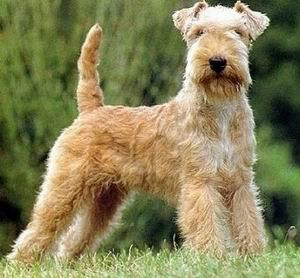
\includegraphics[width=1\linewidth]{Figures/lakeland.jpg}
        \caption{Lakeland\_terrier}
    \end{subfigure}
    \begin{subfigure}{0.35\linewidth}
        \centering
        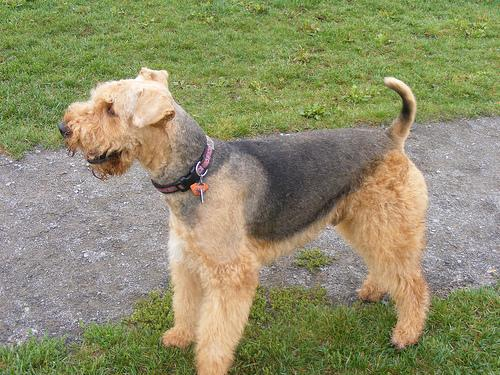
\includegraphics[width=1\linewidth]{Figures/airedale.jpg}
        \caption{Airedale}
    \end{subfigure}
    % ROW END

    % ROW BEGIN
    \begin{subfigure}{0.35\linewidth}
        \centering
        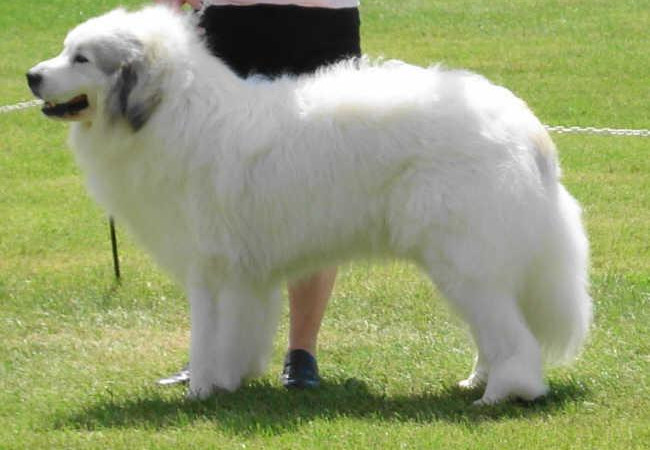
\includegraphics[width=1\linewidth]{Figures/great_pyrenees.jpg}
        \caption{Great\_Pyrenees}
    \end{subfigure}
    \begin{subfigure}{0.35\linewidth}
        \centering
        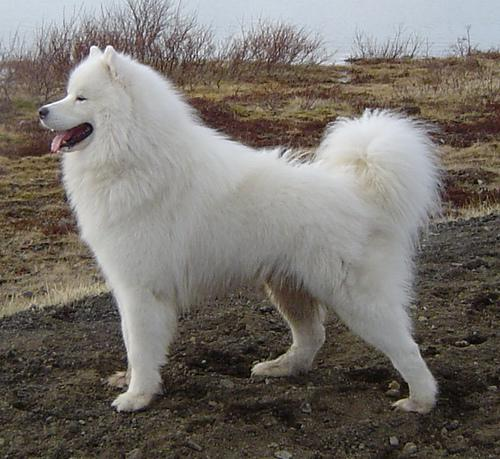
\includegraphics[width=1\linewidth]{Figures/samoyed.jpg}
        \caption{Samoyed}
    \end{subfigure}
    % ROW END

    \caption{Zaměňované psí plemena}
    \label{fig:lukeland_airedale}
\end{figure}

\section{Klasifikace všech psích plemen}
V této sekci bychom se chtěli zabývat klasifikací všech 120 psích plemen, budou tedy využity všechny data z datasetu. Jak jsme již zjistili v kapitole předchozí, počet dat není dostatečný k natrénovaní zcela nové konvoluční neuronové sítě. Z tohoto důvodu hned využijeme techniku \emph{transfer learning}. Co se týče modelů, tak znova využijeme ty, uvedené v Tabulce~\ref{tab:transfered_models}.

Podobně jako u modelu VGG19 v předchozí kapitole, jsme i zde vyzkoušeli větší počet plně propojených vrstev, zde pro model InceptionV3. Výsledky zkoumání úprav modelu InceptionV3 nalezneme v Tabulce~\ref{tab:incv3tests}. V této tabulce jsme zkoušeli několik úprav i augmentaci dat. Všimneme si, že jsme nebyli schopni zlepšit přesnost klasifikace, ale i přesto testovací ztráta klesla oproti základnímu modelu.

\begin{table}[h!]
    \centering
    \begin{tabular}{l | r | r}
    \toprule
    Název                               & Testovací ztráta      & Testovací přesnost  \\\midrule
    Základní model                      & 1,2912                & 0,8501              \\
    Dense512                            & 0,7459                & 0,8367              \\
    2 $\times$ Dense512                 & 0,7989                & 0,8338              \\
    2 $\times$ Dense512 + Dense256      & 0,7278                & 0,8325              \\
    2 $\times$ Dense512 a augmentace    & 0,6262                & 0,8169              \\
    \bottomrule
    \end{tabular}
    \caption{InceptionV3 - úpravy architektury}
    \label{tab:incv3tests}
\end{table}

Podíváme-li se přímo na výsledky převzatých modelů v Tabulce~\ref{tab:transfered_results}, zjistíme že největší přesnosti dosahuje model InceptionResNetV2. Toto jsou pořád výsledky pro obrázky rozměrů $300 \times 300$. Model VGG19 oproti třem ostatním velmi zaostává. Dále se podíváme podrobněji na výsledky nejlepšího modelu. Ten dokázal z 8580 testovacích obrázků správně klasifikovat 7459 obrázků a 1121 tedy bylo špatně zařazeno.

\begin{table}[h!]
    \centering
    \begin{tabular}{l | r }
    \toprule
    Model               & Testovací přesnost  \\\midrule
    VGG19               & 0,2787              \\
    Xception            & 0,8469              \\
    InceptionV3         & 0,8501              \\
    InceptionResNetV2   & 0,8693              \\
    \bottomrule
    \end{tabular}
    \caption{Výsledky klasifikace pro všechny plemena s použitím techniky \emph{transfer learning}}
    \label{tab:transfered_results}
\end{table}

Celá matice záměn bude k dispozici jako příloha, do tohoto textu se nehodí kvůli své velikosti. Co můžeme ale řičí, tak v celé matici se nachází pouze čtyři řádky, kde nalezneme maximální pravděpodobnost mimo hlavní diagonálu. Detaily těchto řádků nalezneme\linebreak v Tabulce~\ref{tab:confmat_mismatch}. U těchto čtyř plemen můžeme očekávat, že ve většině případů dojde ke špatné klasifikaci. Již podle názvu nám dochází, že tyto plemena, správná a zaměňovaná jsou si vizuálně velice podobné.

\begin{table}[h!]
    \centering
    \begin{tabular}{l | l | r | r }
    \toprule
    Správná třída                & Pravď.   & Zaměňovaná třída                            & Pravď. \\\midrule
    Staffordshire\_bullterrier   & 0,2182   & American\_Staffordshire\_terrier      & 0,6909            \\
    Border\_collie               & 0,3200   & collie                                & 0,6000            \\
    Eskimo\_dog                  & 0,3600   & Siberian\_husky                       & 0,4800            \\
    toy\_poodle                  & 0,3333   & miniature\_poodle                     & 0,6666            \\
    \bottomrule
    \end{tabular}
    \caption{Hlavní záměny při klasifikaci všech plemen}
    \label{tab:confmat_mismatch}
\end{table}

Ukázky klasifikací nalezneme na následujících obrázcích. V zeleném obdélníku je vždy uvedena správná třída a v červeném obdélníku je uvedena špatně určena třída. Číslo napravo od názvu plemene značí pravděpodobnost, s jakou byla třída určena. Obrázky správné klasifikace nalezneme na Obrázku~\ref{fig:correct_class}. Zde vidíme, že téměř všechny plemena jsou určena s pravděpodobností 1,0000 nebo alespoň hodně vysokou hodnotou. Ukázka chybných klasifikací je uvedena na Obrázku ~\ref{fig:wrong_class}. Zde už není třída určena s tak velkou pravděpodobností, ale často se stává, že správná třída má dosti malou pravděpodobnost. Toto znamená, že se model nenaučil tyto plemena dobře detekovat. Dalším vysvětlením je málo různých trénovacích dat. 

\image{correct_predictions.pdf}{Ukázka správné klasifikace}{fig:correct_class}{0.8}
\image{wrong_predictions.pdf}{Ukázka špatné klasifikace}{fig:wrong_class}{0.8}

Abychom ještě vylepšili výsledky nejlepšího modelu InceptionResNetV2 vyzkoušeli jsme obrázky zvětšit na $500 \times 500$ pixelů. Díky této úpravě klesla testovací ztráta z 0,9943 na 0,5830 a přesnost vzrostla na 0,8956 z původních 0,8693. Zvětšením rozlišení jsme tedy dosáhli zlepšení v rámci cca 2,5 procenta. Nevýhodou tohoto přístupu je větší paměťová a časová náročnost.

\section{Závěr}
V této práci jsme se zaměřili na klasifikaci psů podle plemen. Z originálního datasetu, který byl rozdělen na trénovací a testovací část jsme natrénovali několik modelů konvolučních neuronových sítí. Snaha o vytvoření a natrénování vlastního modelu byla marná, z důvodu, který bude uveden dále. Hojně jsme v tomto projektu využili techniky \emph{transfer learning}, která nám dovoluje použít a upravit již předem naučené modely. Hlavním problémem originálního datasetu je nedostatek trénovacích dat. Na každé plemeno je k dispozici pouze 100 obrázků a plemen je celkem 120. Tento problém jsme se snažili vyřešit augmentací dat, která avšak nevedla k lepším výsledkům. Co se týče převzatých modelů, tak těch jsme vyzkoušeli čtyři, od jednoduššího VGG19 až po složitý InceptionResNetV2, který kombinuje techniky ze dvou různých architektur. Konvoluční neuronové sítě jsme vyzkoušeli nejdříve na 20 vybraných plemenech, které byly nejvíce zastoupeny v testovacím datasetu. Zde jsme dosáhli velmi vysokých přesností kolem 96 \%. Dále jsme se již vrhli na celou datovou sadu a všech 120 plemen. Zde dosáhli tři převzaté modely přesnosti minimálně 84 \% a nejlepší InceptionResNetV2 dosáhl 86,93 \%. Tento výsledek jsme dokázali ještě o něco málo zlepšit pomocí zvětšení obrázků.


\bibliography{citations}
\bibliographystyle{ieeetr}


\end{document}